\section{Maths for 3D motion}
\subsection{Definitions}
\begin{figure}[h!]
	\centering
	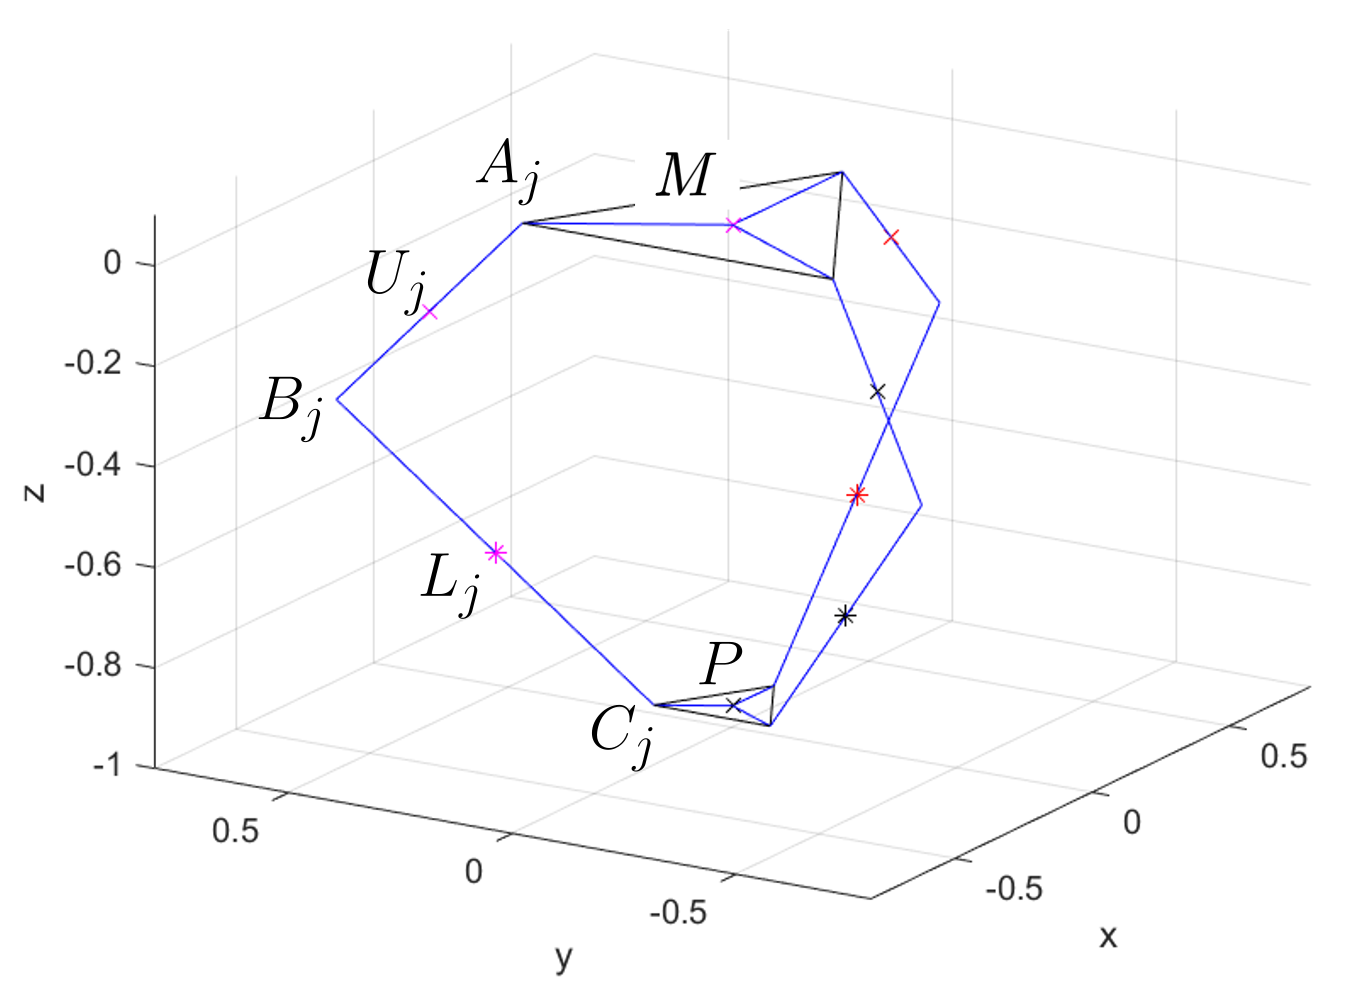
\includegraphics[width=0.7\textwidth]{figures/Initial_3D.png}                                                              
	\caption[Initial configuration of the 3D Delta robot]{Initial configuration of the 3D Delta robot.}
	\label{fig:initia3D}
\end{figure}

Independent and dependent co-ordinates
\begin{align}
q_i&=
\begin{bmatrix}
(\theta_{U,j})_x \\
(\theta_{U,j})_y \\
(\theta_{U,j})_z \\
\vdots
\end{bmatrix} &
q_a&=
\begin{bmatrix}
\theta_{a,1} \\
\theta_{a,2} \\
\theta_{a,3}
\end{bmatrix}
\end{align}

\begin{equation}
\begin{aligned}
\omega^{O,U}_a&=R^O_U \omega^{U,U}_a \\
&=    \begin{bmatrix}
cos(\theta_a) cos(\psi_0) & -sin(\psi_0) & cos(\psi_0) sin(\theta_a) \\
cos(\theta_a) sin(\psi_0) & \hphantom{-} cos(\psi_0) & sin(\psi_0) sin(\theta_a)\\
-sin(\theta_a) & 0 & cos(\theta_a) 
\end{bmatrix}
\begin{bmatrix}
0 \\ \omega_a \\0
\end{bmatrix}\\
&=\begin{bmatrix}
-sin(\psi_0)\omega_a  \\ \hphantom{-} cos(\psi_0)\omega_a   \\0 %\hphantom{-} creates empty space as big as a "-" sign
\end{bmatrix} \\
%\end{aligned}
%\end{equation}
%
%\begin{equation}
%\begin{aligned}
\implies \int \omega^{O,U}_a dt&=\int R^O_U \omega^{U,U}_a dt \\
%\theta_U - \begin{bmatrix} 0\\\theta_{a,0}\\\psi_0 \end{bmatrix}
%&=\begin{bmatrix}
% -sin(\psi_0)\theta_a-\theta_{a,0} \\ cos(\psi_0)\theta_a-\theta_{a,0}  \\0
%  \end{bmatrix}  \
\therefore \theta_U-\theta_{U,0} &= 
\begin{bmatrix} 
-sin(\psi_0)(\theta_a-\theta_{a,0}) \\ \hphantom{-} cos(\psi_0)(\theta_a-\theta_{a,0}) \\ \psi_0
\end{bmatrix}
\end{aligned}
\end{equation}


Constraint equations for the position
\begin{equation}
    \Phi=
    \begin{bmatrix}
    \begin{array}{l} % for proper alignment
    M+R_{A,j}\begin{bmatrix}\frac{L_b}{2} \\ 0 \\0 \end{bmatrix} - U_j - R_{U,j} \begin{bmatrix}0\\ 0 \\\frac{L_u}{2}  \end{bmatrix}  \vspace{0.5em}\\
   %\\
    U_j+R_{U,j}\begin{bmatrix}0 \\ 0 \\-\frac{L_u}{2} \end{bmatrix} - L_j - R_{L,j} \begin{bmatrix}0\\ 0 \\\frac{L_l}{2}  \end{bmatrix}  \vspace{0.5em}\\
    %\\
    L_j+R_{L,j}\begin{bmatrix}0 \\ 0 \\ \frac{-L_l}{2} \end{bmatrix} - P - R_{A,j} \begin{bmatrix}\frac{L_e}{2}\\ 0 \\0 \end{bmatrix}  \vspace{0.5em} \\
    %\\
    \begin{bmatrix} 0 & 1 & 0 \end{bmatrix}R_{L,j}^T(R_{L,j})_0\begin{bmatrix} 1\\ 0 \\0\end{bmatrix}
    \end{array}\\
    %\vdots \\
    \vdots
    %\vdots
    \end{bmatrix},\; j=1,2,3 \label{eq:Phi3D}
\end{equation}

\begin{equation}
    \Phi^{driving}=
    \begin{bmatrix}
    \begin{array}{l} % for proper alignment
    (\theta_{U,j})_x + sin((\theta_{a,j})_0)\omega_j t - 0\\
    (\theta_{U,j})_y - cos((\theta_{a,j})_0)\omega_j t - (\theta_{a,j})_0 \\
    (\theta_{U,j})_z - (\theta_{U,j})_{z,0}
    \end{array}\\
    \vdots
    \end{bmatrix}
\end{equation}

\subsection{Kinematics}
The following is true for all rotation matrices:
\begin{align}
RR^T&=I \\
\implies \dot{R}R^T+R\dot{R^T}&=0 \nonumber\\
\therefore \dot{R}R^T&=-R\dot{R^T}=\tilde{\omega} \label{eq:omega}
\end{align}
Written with reference frame superscripts and subscripts:
\begin{align}
       \dot{R}^O_C &=\tilde{\omega}^O R^O_C \label{eq:Rdot} \\
             &= R^O_C \tilde{\omega}^C \label{eq:Rdot2}
\end{align}

The velocity and acceleration for a point on a rigid body is then:
\begin{align}
r_P^{O,O}&=r_C^{O,O}+R^O_C r_P^{C,C} \\
\implies v_P^{O,O}&=v_C^{O,O}+\dot{R}^O_C r_P^{C,C} \nonumber\\
                 &=v_C^{O,O}+\tilde{\omega}^{O,O}_C R^O_C r_P^{C,C}  \label{eq:Vel3D}\\
\implies a_P^{O,O}&=a_C^{O,O}+\tilde{\alpha}^{O,O}_C R^O_C r_P^{C,C} + \tilde{\omega}^{O,O}_C \dot{R}^O_C r_P^{C,C} \nonumber \\
                  &=a_C^{O,O}+\tilde{\alpha}^{O,O}_C R^O_C r_P^{C,C} + \tilde{\omega}^{O,O}_C \tilde{\omega}^{O,O}_C R^O_C r_P^{C,C} \label{eq:Acc3D}
\end{align}

The following identity is useful:
\begin{align*}
\tilde{\omega}^O R^O_C r^C &= \tilde{\omega}^O r^O \\
                           &= (\tilde{r}^O)^T \omega^O   &&\text{property of anti-symmetric matrices} \\
                           &= R^O_C (\tilde{r}^C)^T R_C^O \omega^O &&\text{equations \ref{eq:Rdot} and \ref{eq:Rdot2}} 
\end{align*}

$\tfrac{d\Phi}{dt}$ can be found using equations \ref{eq:Vel3D} and \ref{eq:Acc3D} and can then be compared with equations \ref{eq:PhiDot} and \ref{eq:Gamma}:
\begin{equation}
\begin{split}
    \frac{d\Phi}{dt}&=
    \begin{bmatrix}
    \begin{array}{cccccc} % for proper alignment
    I & -I & -R_{U,j}({\tilde r}^{U,U}_A)^T R_{U,j}^T & 0 & 0 & ... \\
    0 &  I & +R_{U,j}({\tilde r}^{U,U}_B)^T R_{U,j}^T & -I& -R_{L,j}({\tilde r}^{L,B}_L)^T R_{L,j}^T & ...\\
    0 & 0 & 0 & I & +R_{L,j}({\tilde r}^{L,C}_L)^T R_{L,j}^T & ... \\
    0 & 0 & 0 & 0 & e_{y}^0 R_{L,j}^T \tilde{e}_{x}^{U} & ... 
    \end{array}\\
    \vdots
    \end{bmatrix}
    \begin{bmatrix}
    \dot{M} \\
    \dot{U}_j \\
    \omega_{U,j} \\
    \dot{L}_J \\
    \omega_{L,j} \\
    \vdots
    \end{bmatrix} \label{eq:PhiDot3D}\\
    &=\Phi_q \tfrac{dq}{dt}
\end{split}
\end{equation}


Similarly, for the accelerations

\begin{equation}
\begin{split}
\frac{d^2\Phi}{dt^2}&=
\begin{bmatrix}
\begin{array}{cccccc} % for proper alignment
I & 0 & -R_{U,j}{\tilde r}^{U,U}_A R_{U,j}^T & 0 & 0 & ... \\
0 & I & +R_{U,j}{\tilde r}^{U,U}_B R_{U,j}^T & -I& -R_{L,j}{\tilde r}^{L,B}_L R_{L,j}^T & ...\\
0 & 0 & 0 & I & +R_{L,j}{\tilde r}^{L,C}_L R_{L,j}^T & ... \\
0 & 0 & 0 & 0 & e_{y}^0 R_{L,j}^T \tilde{e}_{x}^{U} & ... 
\end{array}\\
\vdots
\end{bmatrix}
\begin{bmatrix}
\ddot{M} \\
\ddot{U}_j \\
\alpha_{U,j} \\
\dot{L}_J \\
\alpha_{L,j} \\
\vdots
\end{bmatrix} \label{eq:PhiDDot3D}\\
&+
\begin{bmatrix}
\begin{array}{cccccc} % for proper alignment
0 & 0 & -{\tilde{\omega}^{O,O}_{U}}R_{U,j}{\tilde r}^{U,U}_A R_{U,j}^T & 0 & 0 & ... \\
0 & 0 & +{\tilde{\omega}^{O,O}_{U}}R_{U,j}{\tilde r}^{U,U}_B R_{U,j}^T & 0& -{\tilde{\omega}^{O,O}_{L}}R_{L,j}{\tilde r}^{L,B}_L R_{L,j}^T & ...\\
0 & 0 & 0 & 0 & +{\tilde{\omega}^{O,O}_{L}}R_{L,j}{\tilde r}^{L,C}_L R_{L,j}^T & ... \\
0 & 0 & 0 & 0 & e_{y}^0 ({\tilde{\omega}^{O,O}_{L}}R_{L,j} )^T \tilde{e}_{x}^{U} & ... 
\end{array}\\
\vdots
\end{bmatrix}
\begin{bmatrix}
\dot{M} \\
\dot{U}_j \\
\omega_{U,j} \\
\dot{L}_J \\
\omega_{L,j} \\
\vdots
\end{bmatrix} \\
&=\Phi_q \ddot{q} + [\Phi_{q}\tfrac{dq}{dt}]_q\tfrac{dq}{dt} \\
&=\Phi_q \ddot{q}-\gamma
\end{split}
\end{equation}


\subsection{Inverse kinematics}
Add the first 3 rows in equation \ref{eq:Phi3D}:
\begin{equation}
    \begin{aligned}
    r&= R_{L,j}\begin{bmatrix}0\\0\\L_l \end{bmatrix} = R_{A,j}\begin{bmatrix}\frac{L_b-L_e}{2}\\0\\0 \end{bmatrix} - R_{U,j}\begin{bmatrix}0\\0\\L_u  \end{bmatrix} - P  \\
\therefore    r^Tr&=r^TR^TRr &
    \end{aligned}
\end{equation}
\begin{equation}
%\begin{aligned}
%        \left(\left(\frac{L_b-L_e}{2}-L_u sin(\theta_{a,j})\right)cos(\psi_0)-P_x\right)^2 &+ \\
%        \left(\left(\frac{L_b-L_e}{2}-L_usin(\theta_{a,j})\right)sin(\psi_0)-P_y\right)^2 &+\\
%        (-L_ucos(\theta_{a,j})-P_z)^2 &= L_l^2
%\end{aligned}
\begin{split}
\implies L_l^2 =&\left(\left(\tfrac{1}{2}(L_b-L_e)-L_u sin(\theta_{a,j})\right)cos(\psi_0) -P_x\right)^2+ \\       &\left(\left(\tfrac{1}{2}(L_b-L_e)-L_usin(\theta_{a,j})\right)sin(\psi_0)-P_y\right)^2+(-L_ucos(\theta_{a,j})-P_z)^2
\end{split}
\end{equation}
% \begin{equation}
%     \Phi^{IK}=
%     \begin{bmatrix}
%      +\dots\\
%     ...
%     \end{bmatrix}
% \end{equation}

This means the 2D equations \ref{eq:gammaIK} can be used:
\begin{equation}
\begin{aligned}
\tfrac{d^2q_a}{dt^2}&=-\Phi_{q_a}^{-1}([\Phi_{q_a}\tfrac{dq_a}{dt}]_{q_a}\tfrac{dq_a}{dt}+[\Phi_{P}\tfrac{dP}{dt}]_{P}\tfrac{dP}{dt}+2[\Phi_{q_a}\tfrac{dq_a}{dt}]_{P}\tfrac{dP}{dt}+\Phi_P\tfrac{d^2P}{dt^2})\\
&=-\Phi_{q_a}^{-1} (\Phi_{q_aq_a}\tfrac{dq_a}{dt}^2+\Phi_{PP}\tfrac{dP}{dt}^2+2\Phi_{q_aP}\tfrac{dq_a}{dt}\tfrac{dP}{dt}+\Phi_P\tfrac{d^2P}{dt^2}) \\
&=\hphantom{-}\Phi_{q_a}^{-1}\gamma^{IK}
\end{aligned}
\end{equation}

% Computer Torque Control
% \begin{align}
%          J&=\Phi_{q_d}^{-1}\Phi_{q_i} \\
%  \dot{q}_d&=-J\dot{q}_i\\
%   \hat{M}&=M_{ii}+ J^T M_{dd}J\\
%   \hat{Q}&=-J^T Q_{A,d}+J^T M_{dd}\Phi_{q_d}^{-1}\gamma
% \end{align}

References: \cite{Schilder2018} \cite{Hibbeler2013}